\documentclass[uplatex, titlepage]{jsarticle}
\usepackage[dvipdfmx]{graphicx}
\usepackage{float}


\title{通信の基礎01}
\author{C0118005 AM1 秋本 遥基}
\date{}

\begin{document}
\maketitle

\section{目的}

  音声について、デジタルデータを扱う際の性質についてを調査する。音声データについて「サンプリング周波数」「量子化ビット数」がファイルの容量及び音声データの音質にどのような変化をもたらすかを観測する。

\section{音の高さと周波数}
【結果】\\
  WaveSpectraを用いて,音声ファイルから一般的な西洋音楽で用いられる「ドレミファソラシド」の音階の$\sharp$を含めた音の周波数を調べた。結果を以下の表\ref{table:oto}に示す。 \\

\begin{table}[H]
  \centering
  \caption{音名と周波数の関係}
  \label{table:oto}
  \begin{tabular}{|l|c|}\hline
    音名 & 周波数[Hz] \\ \hline
    ド & $522.9$ \\ \hline
    ド$\sharp$ & $555.2$ \\ \hline
    レ & $586.8$ \\ \hline
    レ$\sharp$ & $621.8$ \\ \hline
    ミ & $658.8$ \\ \hline
    ファ & $697.8$ \\ \hline
    ファ$\sharp$ & $740.2$ \\ \hline
    ソ & $783.9$ \\ \hline
    ソ$\sharp$ & $829.7$ \\ \hline
    ラ & $880.2$ \\ \hline
    ラ$\sharp$ & $932.0$ \\ \hline
    シ & $987.8$ \\ \hline
    ド+ & $1045.7$ \\ \hline
  \end{tabular}
\end{table}

  この結果より$\sharp$を含めた隣り合う音同士の比較をする。ここではドとド$\sharp$、ド$\sharp$とレ、シとド$\sharp$の比較をした。\\

\begin{table}[H]
  \centering
  %\caption{隣り合う音同士の周波数の関係}
  %\label{table:tonari}
  %\renewcommand{\arraystretch}{2.0}
  \begin{tabular}{cc}%\hline
  計算式 & 有効数字三桁の結果\\ %\hline
  ド$\sharp$ / ド & 1.06\\ %\hline
  レ\ \ /\ ド$\sharp$ & 1.06\\ %\hline
  ド+ / シ & 1.06\\ %\hline
  \end{tabular}
\end{table}

【考察】\\
  結果より、有効数字を任意の精度に絞った際、音の高さに関わらず隣り合った音同士であれば全く同様の結果が得られた。隣り合う音であれば、高い音はおおよそ低い音の周波数を1.06倍した周波数となる。

\section{純音と複合音}

  サイン波、矩形波、三角波、音楽データのスペクトラムを比較し、含まれている周波数にどのような違いがあるか調べる。また、500Hz矩形波の主要三成分を記録し、生成される波形をキャプチャ及び観測する。\\ \\
【結果】\\
  サイン波、矩形波、三角波、音楽データの波形とスペクトラムを以下に示す。\\
%sin squ tri
\begin{figure}[H]
    \begin{tabular}{c}

      \begin{minipage}{0.45\hsize}
        \begin{center}
          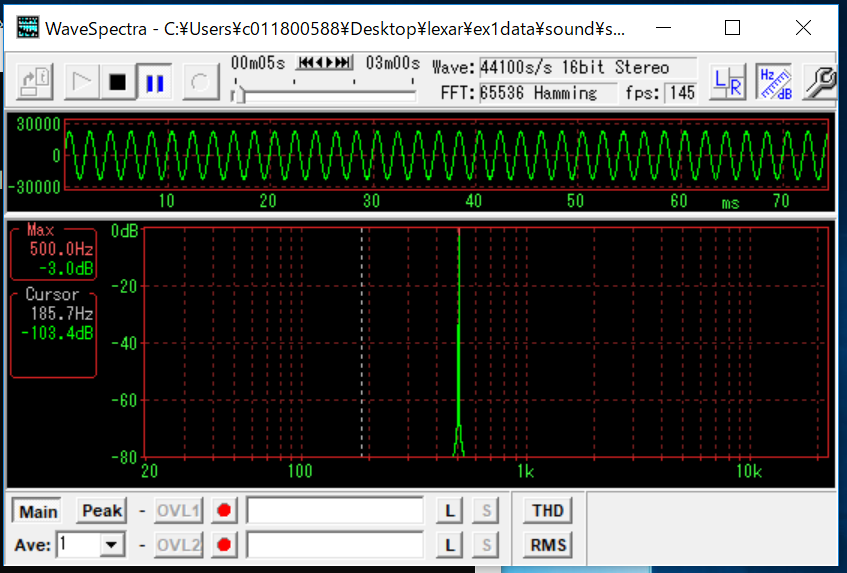
\includegraphics[scale=0.45]{./tuusin1.2/sin.png}
          \caption{500[Hz] サイン波}
          \label{fig:sin}
        \end{center}
      \end{minipage}

      \begin{minipage}{0.45\hsize}
        \begin{center}
          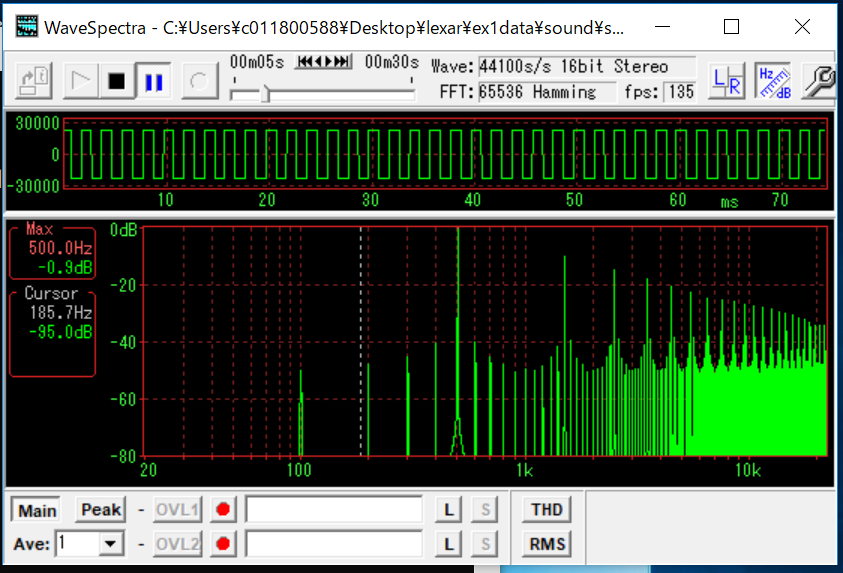
\includegraphics[scale=0.45]{./tuusin1.2/square500.png}
          \caption{500[Hz] 矩形波}
          \label{fig:squ}
        \end{center}
      \end{minipage}

    \end{tabular}
\end{figure}

\begin{figure}[H]
    \begin{tabular}{c}

      \begin{minipage}{0.45\hsize}
        \begin{center}
          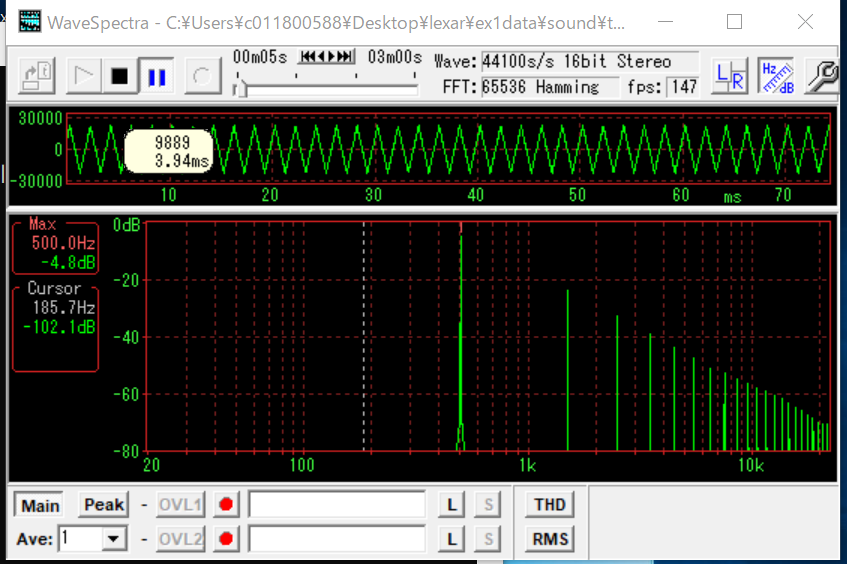
\includegraphics[scale=0.45]{./tuusin1.2/triangle500.png}
          \caption{500[Hz] 三角波}
          \label{fig:tri}
        \end{center}
      \end{minipage}

    \end{tabular}
\end{figure}


%cd
\begin{figure}[H]
    \begin{tabular}{c}

      \begin{minipage}{0.45\hsize}
        \begin{center}
          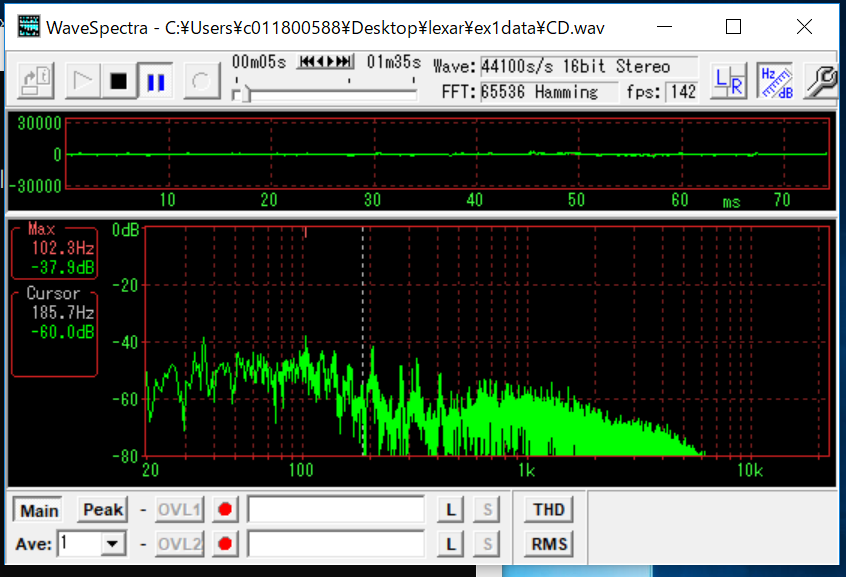
\includegraphics[scale=0.45]{./tuusin1.2/cd01.png}
          \caption{音楽データの波形1}
          \label{fig:cd01}
        \end{center}
      \end{minipage}

      \begin{minipage}{0.45\hsize}
        \begin{center}
          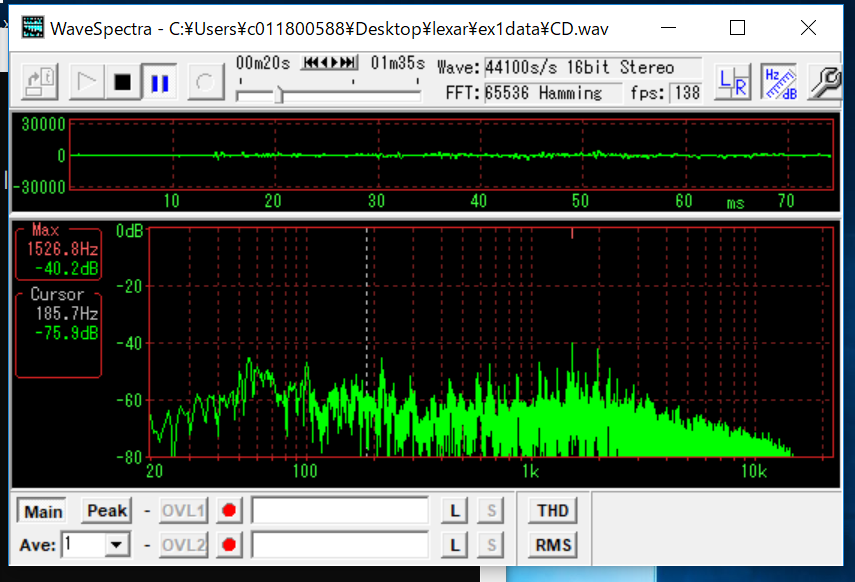
\includegraphics[scale=0.45]{./tuusin1.2/cd02.png}
          \caption{音楽データの波形2}
          \label{fig:cd02}
        \end{center}
      \end{minipage}

    \end{tabular}
\end{figure}

  また、500Hz矩形波の主要三成分を表\ref{table:500hz}、それらを合成して生成した波形を以下に示す。\\

\begin{table}[H]
  \centering
  \caption{500[Hz]矩形波の主要3成分}
  \label{table:500hz}
  \begin{tabular}{|c|c|c|c|} \hline
    周波数[Hz] & 500 & 1500 & 2500 \\ \hline
    振幅[dB] & -0.9 & -10.5 & -15.1 \\ \hline
  \end{tabular}

\end{table}


\begin{figure}[H]
    \begin{tabular}{c}

      \begin{minipage}{0.45\hsize}
        \begin{center}
          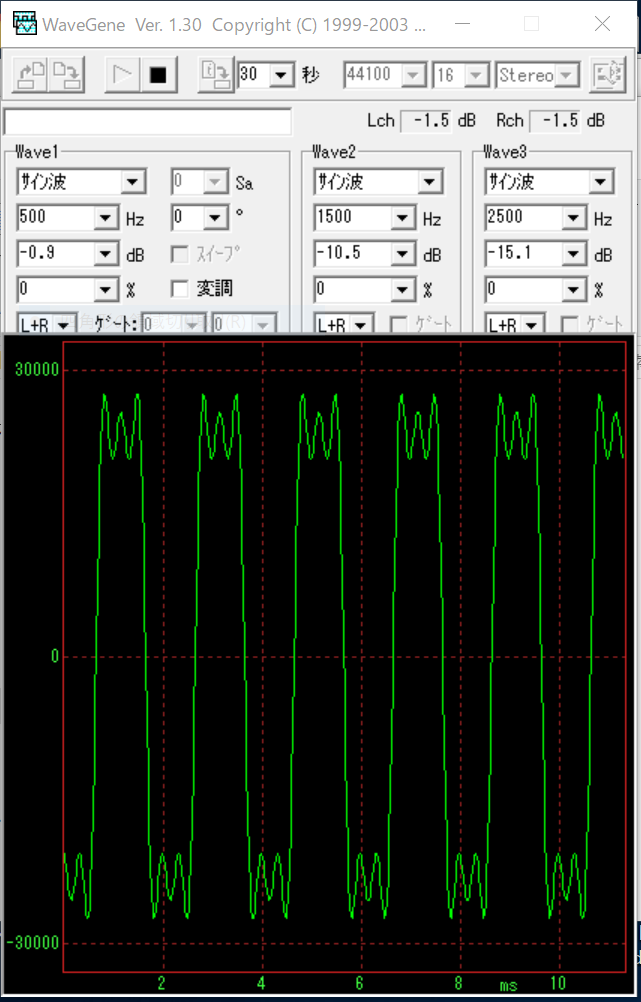
\includegraphics[scale=0.45]{./tuusin1.2/sqmake00.png}
          \caption{主要2成分で生成された波形}
          \label{fig:sqmake00}
        \end{center}
      \end{minipage}

      \begin{minipage}{0.45\hsize}
        \begin{center}
          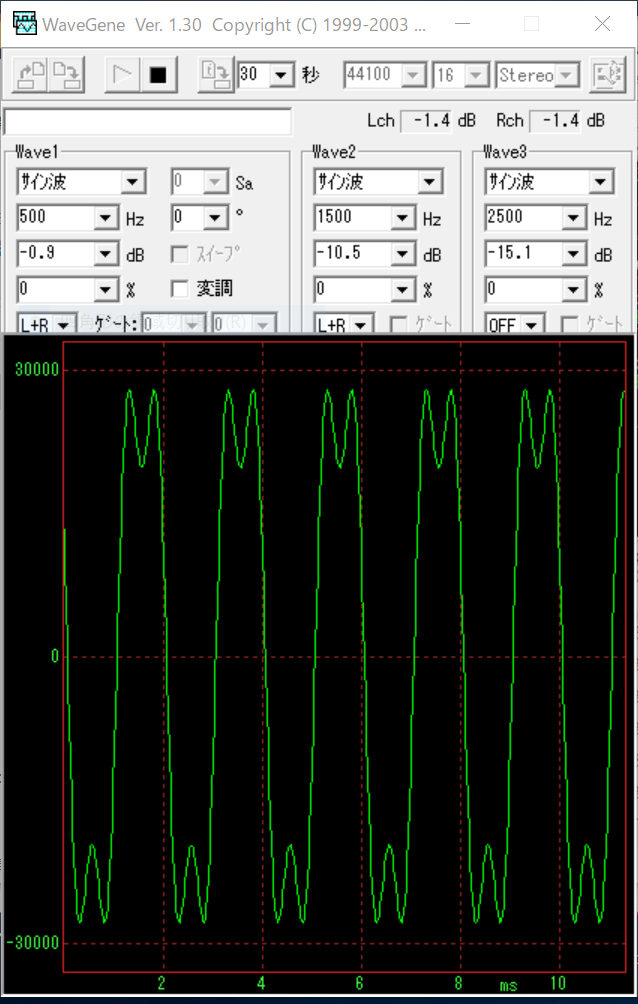
\includegraphics[scale=0.45]{./tuusin1.2/sqmake01.png}
          \caption{主要3成分で生成された波形}
          \label{fig:sqmake01}
        \end{center}
      \end{minipage}

    \end{tabular}
\end{figure}

【考察】

(1)図で示したサイン波(図\ref{fig:sin})は定常的に同様の波形を繰り返しておりサイン波であるため純音である。また矩形波(図\ref{fig:squ})、三角波(図\ref{fig:tri})は一つの正弦波だけでは表せないため複合音であると考えられる。 \\
(2)図で示した音楽データ(図\ref{fig:cd01},図\ref{fig:cd02})は、いずれも時間ごとに全く異なる形状の波形であるため複合音であると考えられる。また二枚のキャプチャ画像はキャプチャ範囲によって全く形が異なっている。これは音楽データは一定の波形ではなく変位する音楽であるため、キャプチャする場所によって波形の形が逐次異なっているからである。\\
(3)これ(図\ref{fig:sqmake00},図\ref{fig:sqmake01})において、2つの波形を比較すると振幅の最大の部分において三つの波形を合成したものの方がより矩形波に近い形をとっている(端点がより平らである)ことにより、合成する周波数成分が多ければ多いほど矩形波の構造に近づいていくと考えられる。\\

\section{サンプリング定理と折り返し}

  各周波数の波形を観測した。以下にサンプリング後の波形と対応する波形の正弦波の周波数及び、その画像を示す。 \\

【結果】
\begin{table}[H]
  \centering
  \caption{サンプリング後の波形と同様になる周波数}
  \label{table:curve}
  \begin{tabular}{|c|c|} \hline
    目的の波形 & サンプリング後の波形 \\ \hline
    0.5 [kHz] & 7.5 [kHz] \\ \hline
    1.0 [kHz] & 7.0 [kHz] \\ \hline
    2.0 [kHz] & 6.0 [kHz] \\ \hline
    3.0 [kHz] & 5.0 [kHz] \\ \hline
  \end{tabular}
\end{table}

\begin{figure}[H]
    \begin{tabular}{c}

      \begin{minipage}{0.45\hsize}
        \begin{center}
          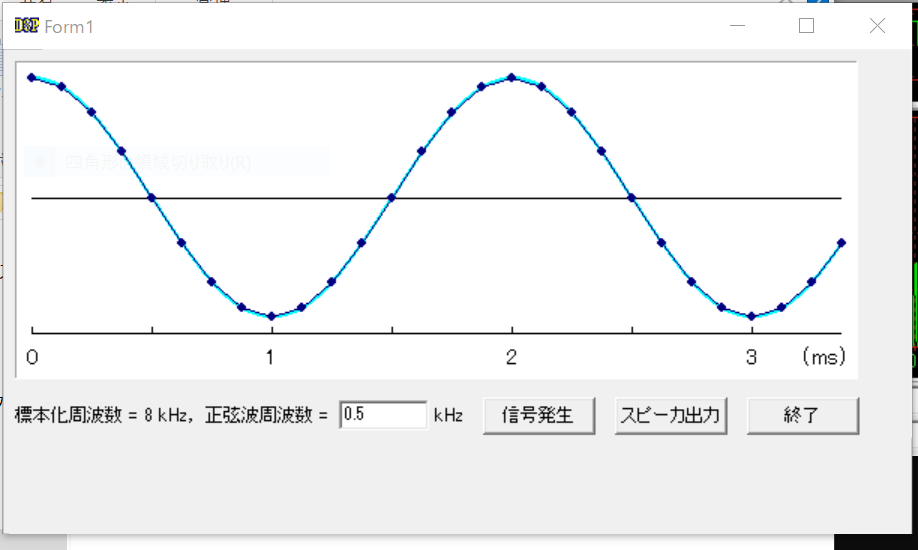
\includegraphics[scale=0.4]{./tuusin1.3/sin05.png}
          \caption{0.5 [kHz]の波形}
          \label{fig:sin05}
        \end{center}
      \end{minipage}

      \begin{minipage}{0.45\hsize}
        \begin{center}
          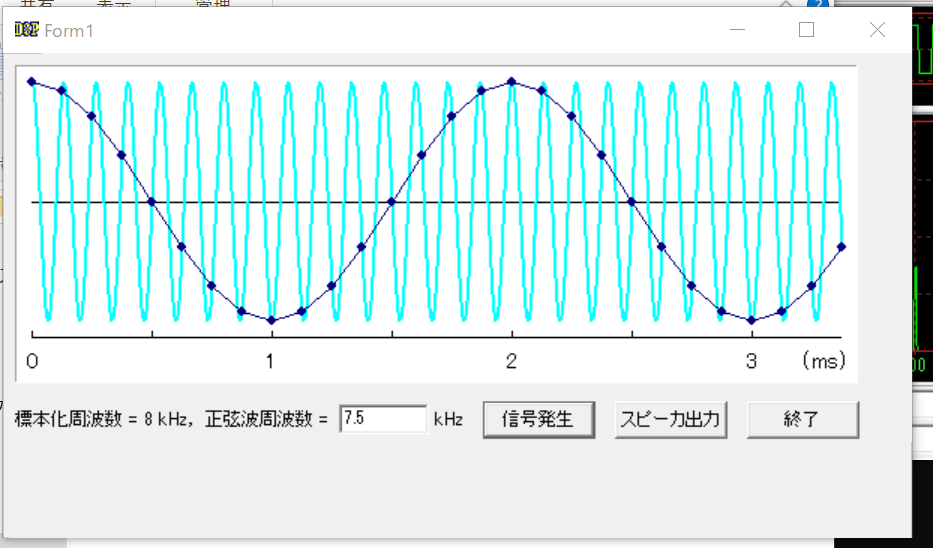
\includegraphics[scale=0.4]{./tuusin1.3/sin75.png}
          \caption{7.5 [kHz]の波形}
          \label{fig:sin75}
        \end{center}
      \end{minipage}

    \end{tabular}
\end{figure}

\begin{figure}[H]
    \begin{tabular}{c}

      \begin{minipage}{0.45\hsize}
        \begin{center}
          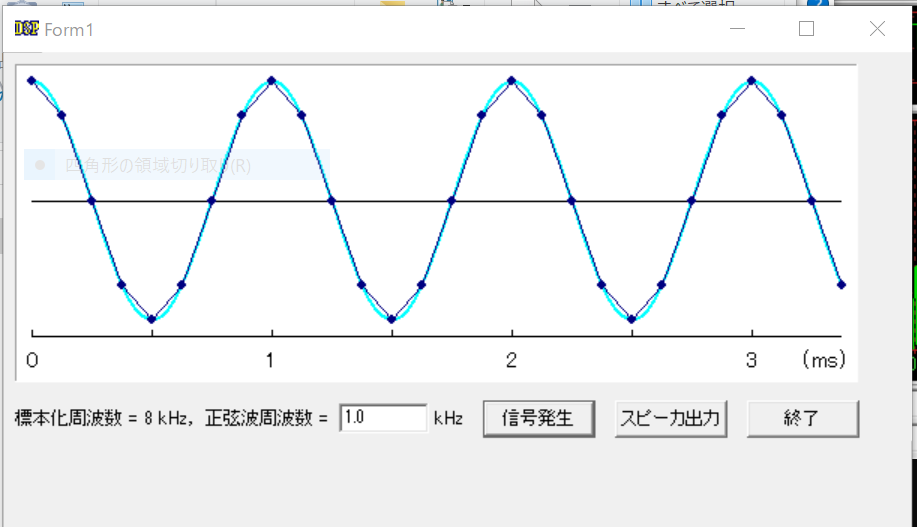
\includegraphics[scale=0.4]{./tuusin1.3/sin10.png}
          \caption{1.0 [kHz]の波形}
          \label{fig:sin10}
        \end{center}
      \end{minipage}

      \begin{minipage}{0.45\hsize}
        \begin{center}
          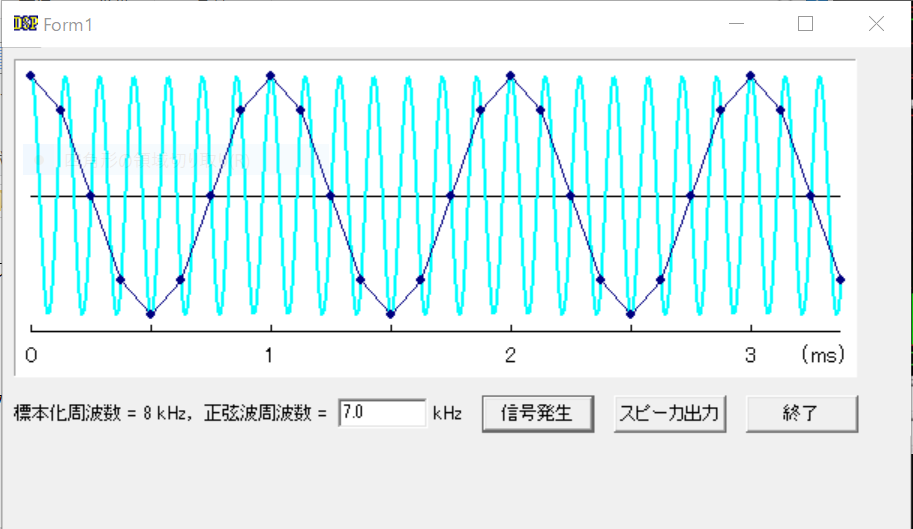
\includegraphics[scale=0.4]{./tuusin1.3/sin70.png}
          \caption{7.0 [kHz]の波形}
          \label{fig:sin70}
        \end{center}
      \end{minipage}

    \end{tabular}
\end{figure}

\begin{figure}[H]
    \begin{tabular}{c}

      \begin{minipage}{0.45\hsize}
        \begin{center}
          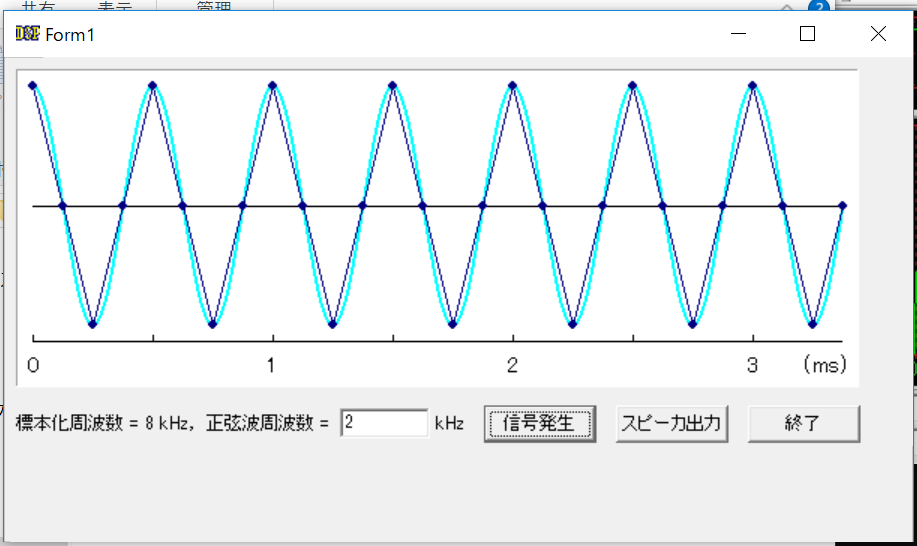
\includegraphics[scale=0.4]{./tuusin1.3/sin20.png}
          \caption{2.0 [kHz]の波形}
          \label{fig:sin20}
        \end{center}
      \end{minipage}

      \begin{minipage}{0.45\hsize}
        \begin{center}
          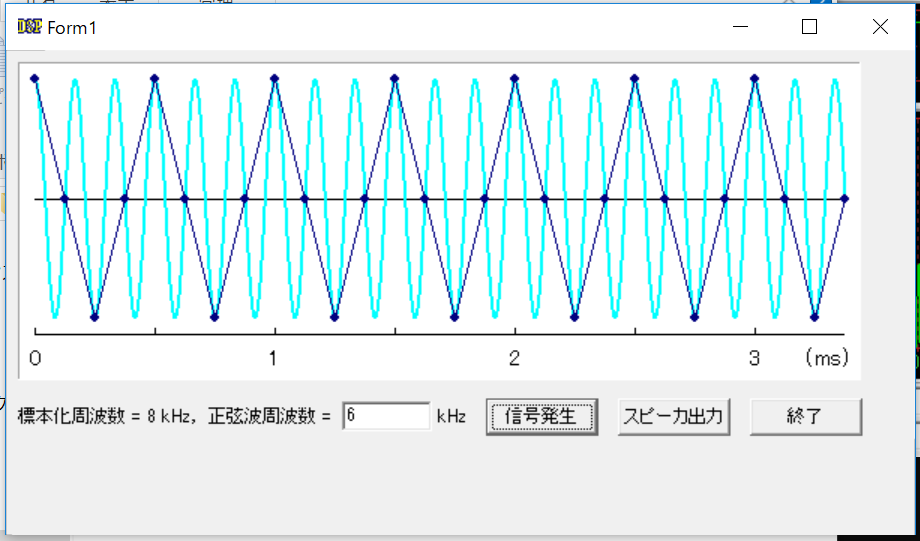
\includegraphics[scale=0.4]{./tuusin1.3/sin60.png}
          \caption{6.0 [kHz]の波形}
          \label{fig:sin60}
        \end{center}
      \end{minipage}

    \end{tabular}
\end{figure}

\begin{figure}[H]
    \begin{tabular}{c}

      \begin{minipage}{0.45\hsize}
        \begin{center}
          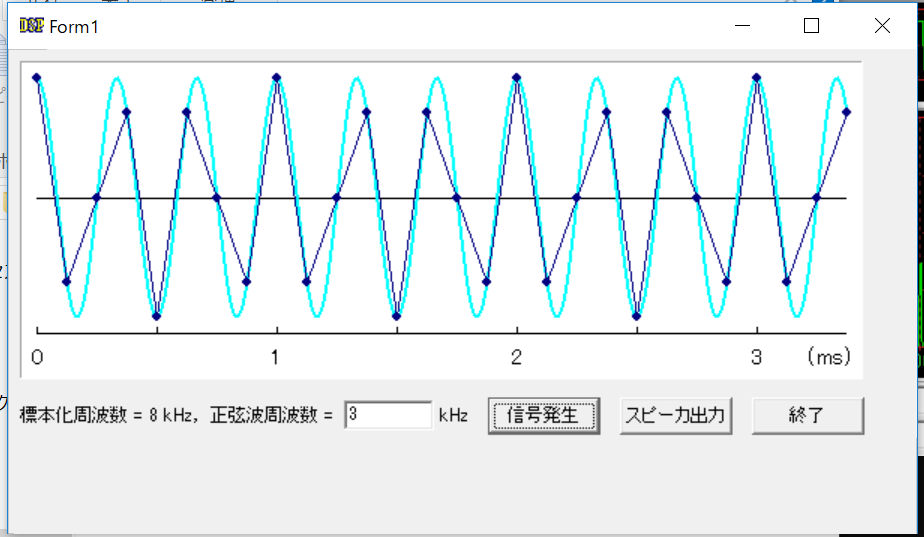
\includegraphics[scale=0.4]{./tuusin1.3/sin30.png}
          \caption{3.0 [kHz]の波形}
          \label{fig:sin50}
        \end{center}
      \end{minipage}

      \begin{minipage}{0.45\hsize}
        \begin{center}
          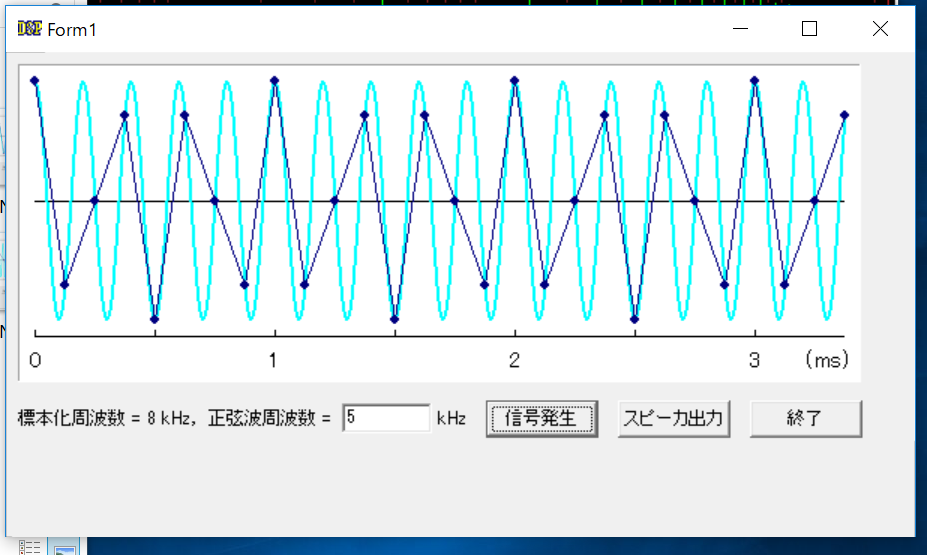
\includegraphics[scale=0.4]{./tuusin1.3/sin50.png}
          \caption{5.0 [kHz]の波形}
          \label{fig:sin50}
        \end{center}
      \end{minipage}

    \end{tabular}
\end{figure}

%\newpage
【考察】\\
(1)サンプリング定理(標本化定理)\cite{one}とは結果の表\ref{table:curve}からわかる通り、サンプリング後の波形を\\$(標本化周波数) - (一致させたい波形の周波数)$とし求めると、同様の形状を持つ波形が得られるものである。\\
(2)サンプリング周波数が8kHzであるとき、折り返し周波数は4kHzである。関係性はサンプリング周波数を$f_s$、折り返し周波数を$f_n$とすると、$f_n = \frac{f_s}{2}$という関係性にある。

\section{量子化雑音}

  量子化ビット数を1から15の範囲で変化させたファイルを用意し、聴き比べた。\\
【結果】\\
 音質変化が初めて判別できるビット数は9、音質の劣化が不快になるビット数は7であった。\\
以下に波形の比較をした図を示す。

\begin{figure}[H]
  \centering
  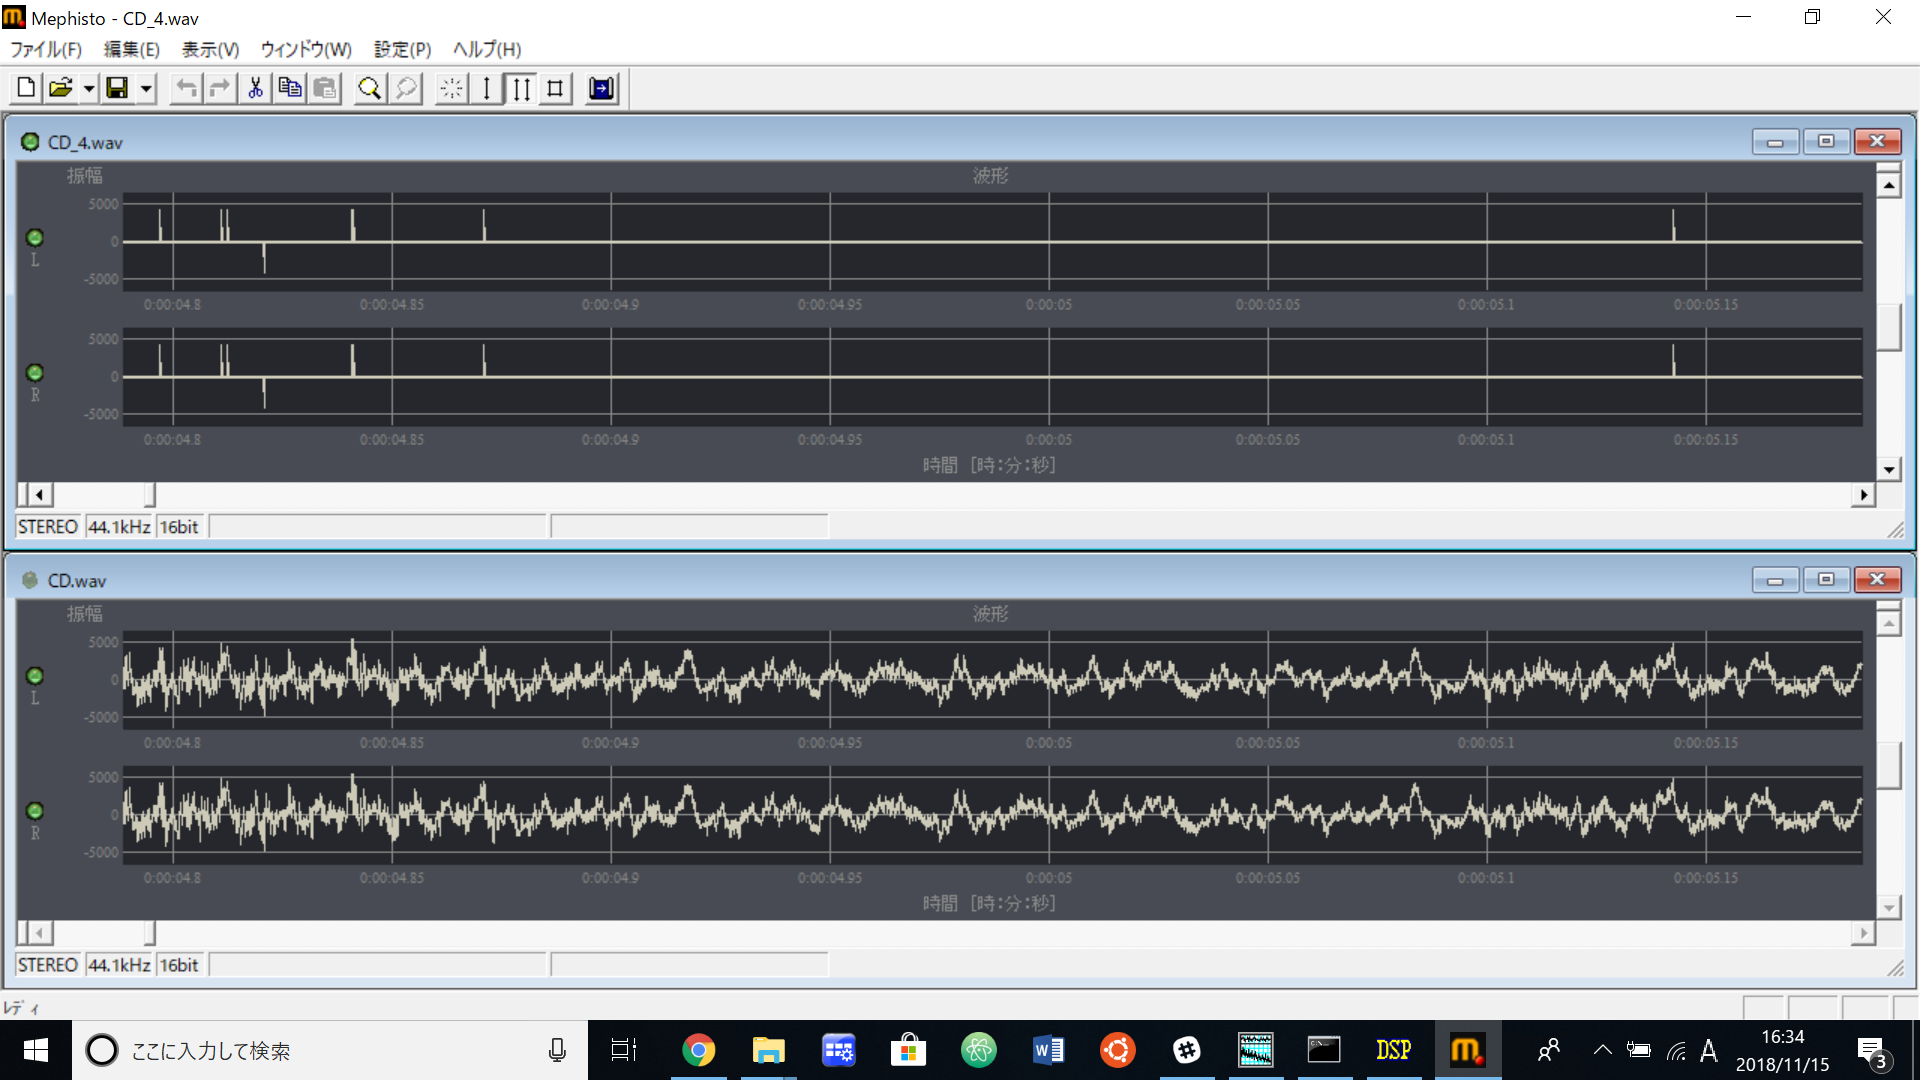
\includegraphics[scale=0.4]{./tuusin1.4/diff4.png}
  \caption{オリジナル波形と量子化ビット数4bitの波形}
  \label{fig:4bit}
\end{figure}

\begin{figure}[H]
  \centering
  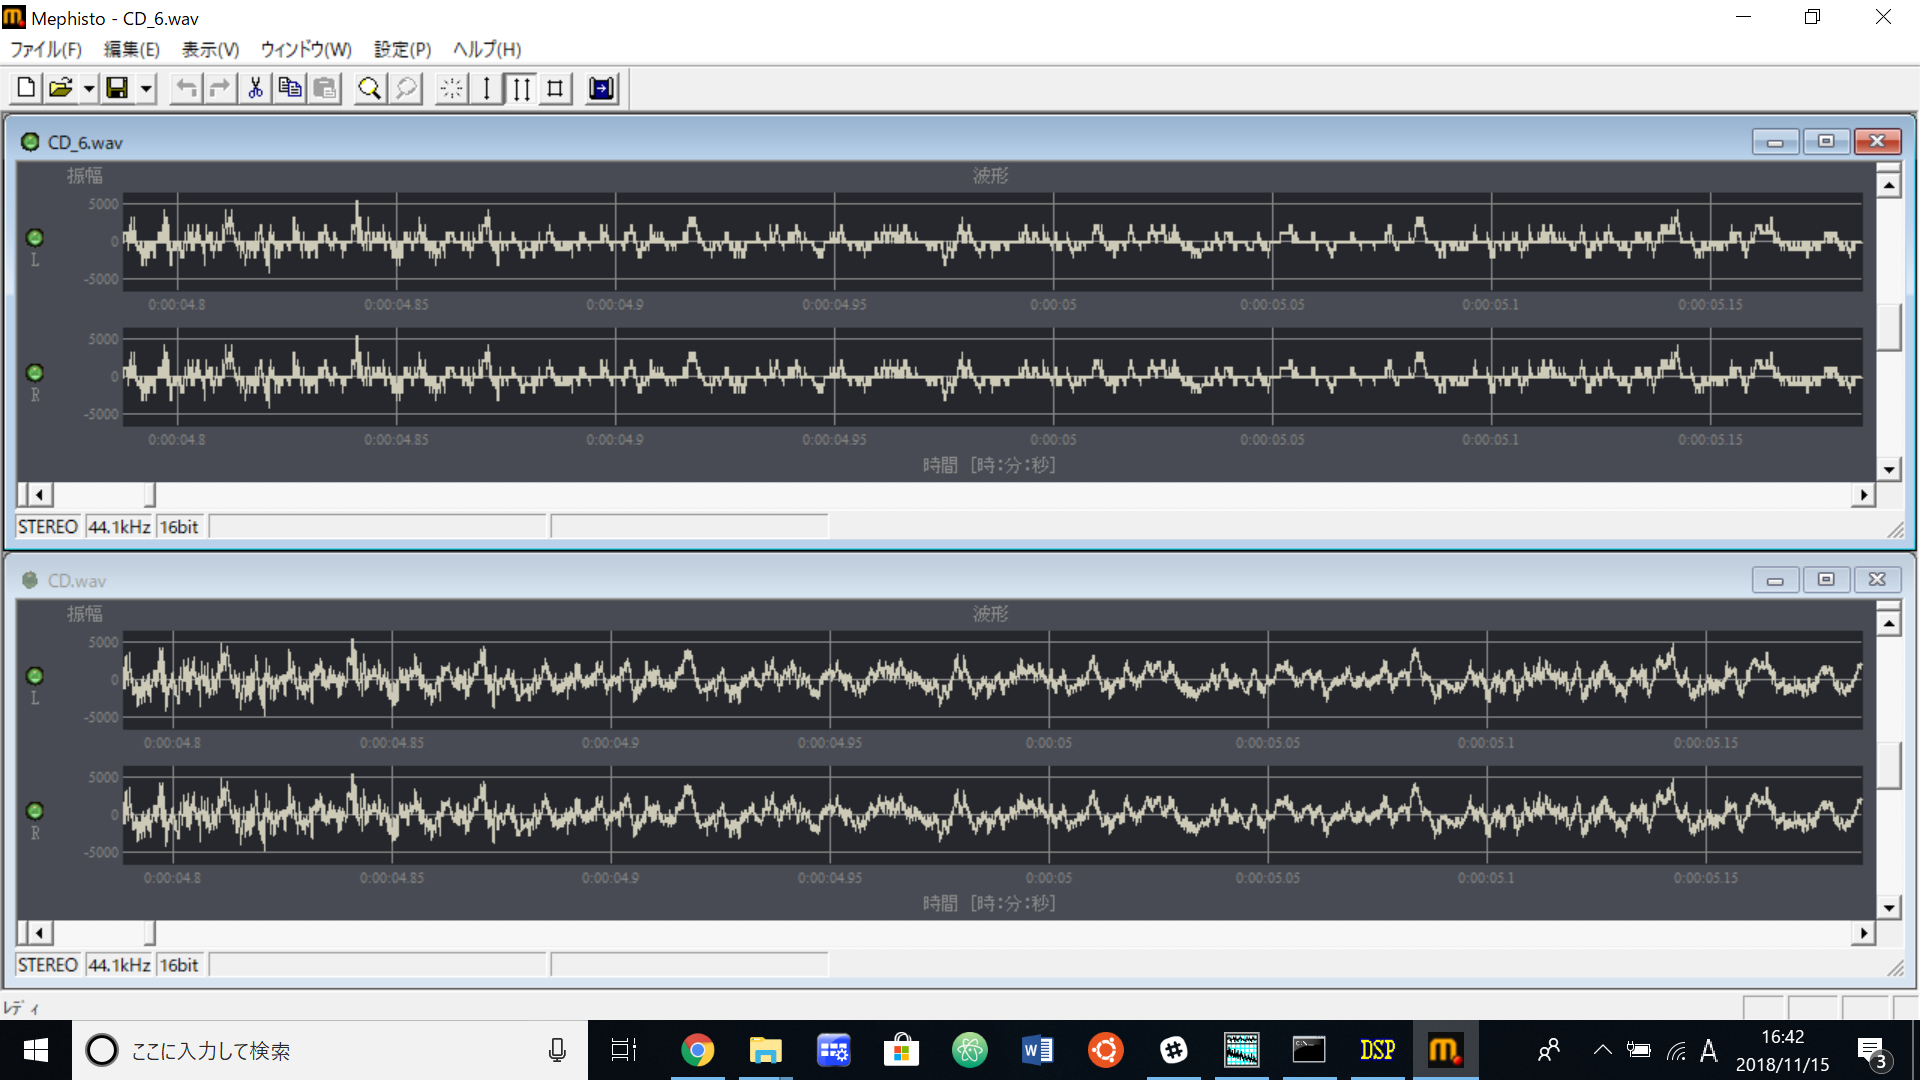
\includegraphics[scale=0.4]{./tuusin1.4/diff6.png}
  \caption{オリジナル波形と量子化ビット数6bitの波形}
  \label{fig:6bit}
\end{figure}

\begin{figure}[H]
  \centering
  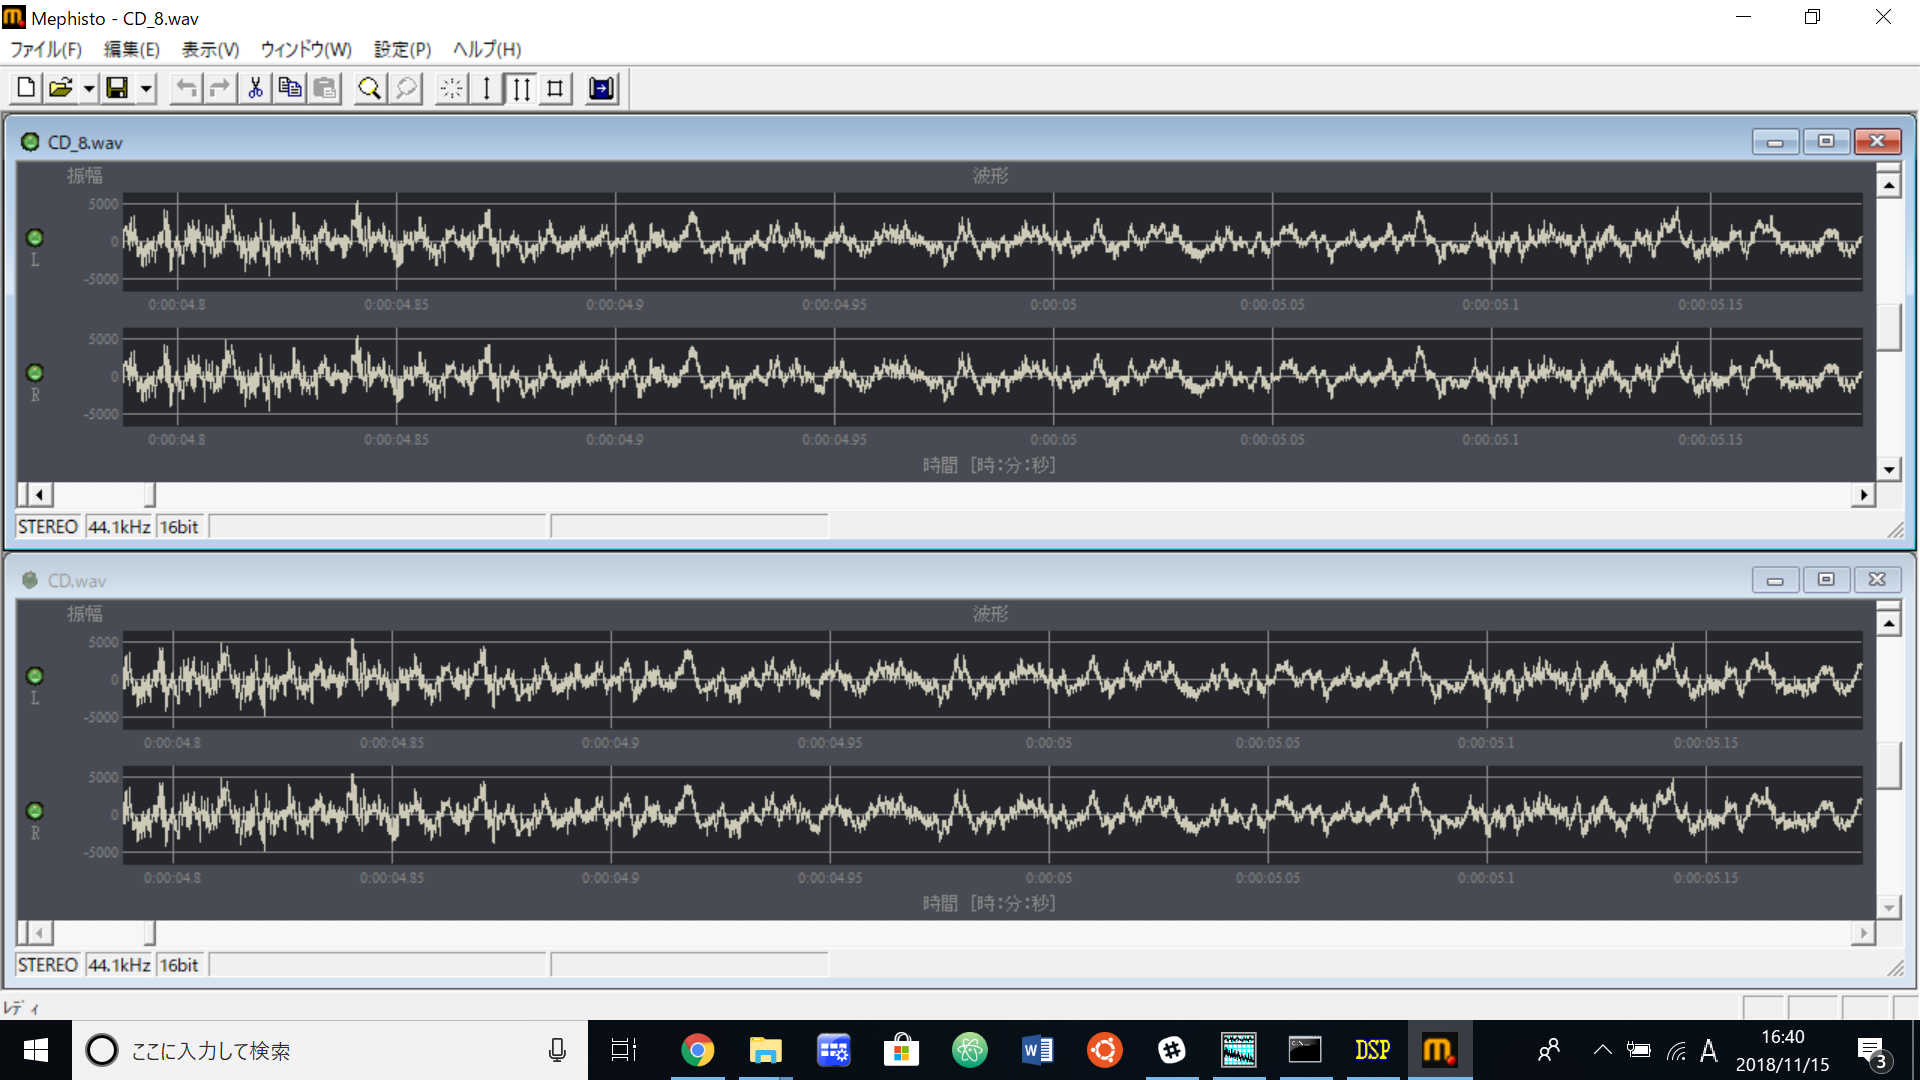
\includegraphics[scale=0.4]{./tuusin1.4/diff8.png}
  \caption{オリジナル波形と量子化ビット数8bitの波形}
  \label{fig:8bit}
\end{figure}

【考察】\\
  量子化ビット数を小さくすると音質が悪くなった。これは量子化ビット数を小さくするにつれ(図\ref{fig:4bit},図\ref{fig:6bit},図\ref{fig:8bit})より、波形の情報量が減り劣化したためと考えられる。

%\newpage

\section{サンプリング周波数変換}

  サンプリング周波数を変化させた音声ファイルを生成した。以下に結果の表\ref{table:filesamp}を示す。\\

【結果】
\begin{table}[H]
  \centering
  \caption{サンプリング周波数とファイルサイズ}
  \label{table:filesamp}
  \begin{tabular}{|c|c|} \hline
    サンプリング周波数[Hz] & ファイルサイズ[バイト] \\ \hline
    8000 & 3041158 \\ \hline
    11025 & 4191074 \\ \hline
    22050 & 8382094 \\ \hline
    44100 & 16764134 \\ \hline
  \end{tabular}
\end{table}

  この表\ref{table:filesamp}より、グラフを作成した。この際、結果に原点データを付け加えた。以下にこれを示す。

\begin{figure}[H]
  \centering
  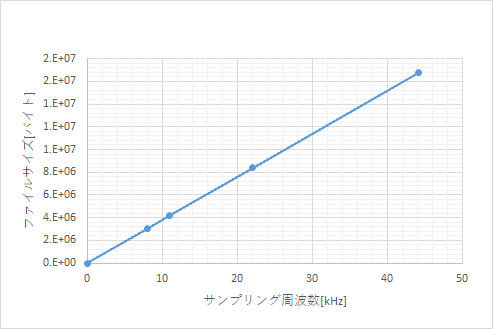
\includegraphics[scale=1.3]{./tuusin1.4/gra.png}
  \caption{サンプリング周波数とファイルサイズの関係}
  \label{graphicx:last}
\end{figure}

【考察】\\
(1)各サンプリング周波数より、再生可能な周波数の上限を求めた。以下の表\ref{table:last}に示す。

\begin{table}[H]
  \centering
  \caption{再生可能な周波数の上限}
  \label{table:last}
  \begin{tabular}{|c|c|c|c|c|} \hline
    サンプリング周波数[Hz] & 44100 & 22050 & 11025 & 8000 \\ \hline
    再生周波数の上限[Hz] & 22050 & 11025 & 5512 & 4000 \\ \hline
  \end{tabular}
\end{table}

(2)サンプリング周波数を下げたときの各音楽データを聞くと、音の明瞭さが下がるということが分かった。この変化は、再生周波数の上限が減ったことにより、波形の情報量が減少したためと考えられる。

\begin{thebibliography}{99}
  \bibitem{one} \verb+"音の性質とサンプリング、量子化",https://service.cloud.teu.ac.jp/lecture/CSF+
  \verb+/kinoshi/%E9%80%9A%E4%BF%A1%E3%81%AE%E5%9F%BA%E7%A4%8E/1.Sound(Sampling,Quantization).pdf,+
  (参照:\today)
  \end{thebibliography}
\end{document}
